\documentclass[10pt,a4paper]{article}
\usepackage[margin=0.5in]{geometry}
\usepackage[utf8]{inputenc}
\usepackage[english]{babel}
\usepackage{amsmath}
\usepackage{amsfonts}
\usepackage{amssymb}
 \usepackage{cancel}
\usepackage{graphicx}

\title{Solid angle subtended by a tetrahedron computation}
\begin{document}

\maketitle


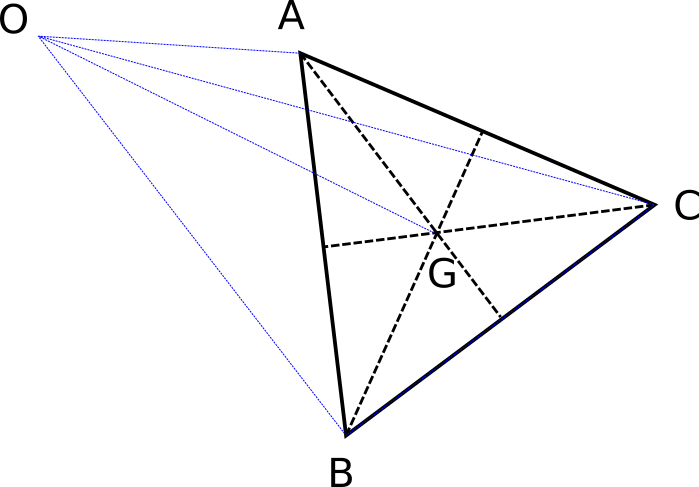
\includegraphics[scale=0.4]{tetra.png} 


\section{Notations}

Let

\begin{itemize}
	\item $A$ be the vector $\vec{OA}$
	\item $B$ be the vector $\vec{OB}$
	\item $C$ be the vector $\vec{OC}$
	\item $a$ be the vector $\vec{GA}$
	\item $b$ be the vector $\vec{GB}$
	\item $c$ be the vector $c$
	\item $\mathbf{A}$ be the magnitude of the vector $\vec{OA}$
	\item $\mathbf{B}$ be the magnitude of the vector $\vec{OB}$
	\item $\mathbf{C}$ be the magnitude of the vector $\vec{OC}$
\end{itemize}

\section{Computation}

The solid angle $\Omega$ subtended by the triangular surface $ABC$ is:

$$
{\displaystyle \tan \left({\frac {1}{2}}\Omega \right)
  = {\frac {\left|{A}\ {B}\ {C}\right|}
    {\mathbf{A}\mathbf{B}\mathbf{C} + \left({A}\cdot {B}\right)\mathbf{C}
      + \left({A}\cdot {C}\right)\mathbf{B}
      + \left({B}\cdot {C}\right)\mathbf{A}}}}
$$

where $ \left|{A}\ {B}\ {C}\right|={A}\cdot ({B}\times {C}) $


\subsection{Numerator}


Given that $A = \vec{OA} = G + a$ (and resp.
with $B$ and $C$), we get


\begin{align*}
\left|{A}\ {B}\ {C}\right|
	& =  {A} \cdot ({B}\times {C}) \\
	& =  {A} \cdot ({(G + b)} \times {(G + c)}) \\
	& =  {(G + a)} \cdot (\cancel{G \times G}
	                      + G \times c
	                      + b \times G
	                      + b \times c) \\
	& = \cancel{G \cdot (G \times c)}
	                      + \cancel{G \cdot (b \times G)}\\
         & + G \cdot (b \times c)
	  + a \cdot (G \times c)
	  + a \cdot (b \times G)
	  + \cancel{a \cdot (b \times c)} \\
	& = G \cdot (b \times c)
	+ G \cdot (c \times a)
	+ G \cdot (a \times b) \\
	& = G \cdot \left(b \times c
	+c \times a
	+ a \times b \right)
\end{align*}

since $G$ is the centroid of $ABC$, 

\begin{equation}
a + b + c= 0
\label{eq1}
\end{equation}. We obtain

\begin{align}
\left|{A}\ {B}\ {C}\right|
& = G \cdot \left(b \times c
	+c \times a
	+ a \times b \right) \nonumber \\
& = G \cdot \left(b \times c
	+c \times (-b - c)
	+ (-b - c) \times b \right) \nonumber \\
& = G \cdot \left(b \times c
	+c \times (-b) + \cancel{c \times (- c)}
	+ \cancel{(-b) \times b} + (- c) \times b \right) \nonumber \\
& = G \cdot \left(3 b \times c \right) \nonumber \\
& = 3 G \cdot \left( b \times c \right)
\end{align}

\subsection{Denominator}


First let's see the term in $\mathbf{C}$
\begin{align*}
 \left({A}\cdot {B}\right)\mathbf{C}
	=& \left( G + a \right) \cdot \left( G + b \right) \mathbf{C} \\
	 =& (\mathbf{G}^2 +  G \cdot b	+ a \cdot G + a \cdot b    ) \mathbf{C}
\end{align*}

Using \eqref{eq1}

\begin{align}
 \left({A}\cdot {B}\right)\mathbf{C}
	 =& (\mathbf{G}^2 +  G \cdot b	+ (-b - c) \cdot G + (-b - c) \cdot b    ) c \nonumber \\
	 =& (\mathbf{G}^2 - ||GB||^2 - G \cdot c - c \cdot b)\mathbf{C}
\end{align}



Now, the term in $\mathbf{B}$


\begin{align*}
 \left({A}\cdot {C}\right)\mathbf{B} 
	=& \left( G + a \right) \cdot \left( G + c \right) \mathbf{B} \\
	 =& (\mathbf{G}^2 +  G \cdot c	+ a \cdot G + a \cdot c    ) \mathbf{B}
\end{align*}

Using \eqref{eq1}

\begin{align}
 \left({A}\cdot {C}\right)\mathbf{B}
	 =& (\mathbf{G}^2 +  G \cdot c	+ (-b - c) \cdot G + (-b - c) \cdot c    ) b \nonumber \\
	 =& (\mathbf{G}^2 - ||GC||^2 - G \cdot c - c \cdot b)\mathbf{B}
\end{align}


For the third term there is no simplification

\begin{align}
 \left({B}\cdot {C}\right)\mathbf{A}
	=& \left( G + b \right) \cdot \left( G + c \right) \mathbf{A}
\end{align}


For the computation of the norms, we can use:

\begin{align*}
\mathbf{A}^2 &= ||OG||^2 + \mathbf{a}^2 - 2 G \cdot a \\
        &=  \mathbf{G}^2 + \mathbf{a}^2 - 2 G \cdot a 
\end{align*}

and respectively with B and C, we obtain


\begin{align}
(\mathbf{A}\mathbf{B}\mathbf{C})^2 &= (\mathbf{G}^2 + \mathbf{a} - 2 G \cdot a )^2(\mathbf{G}^2 + \mathbf{b} - 2 G \cdot b)^2(\mathbf{G}^2 + \mathbf{c} - 2 G \cdot c)^2 
\end{align}


\section{Final formula}


$$
{\displaystyle \tan \left({\frac {1}{2}}\Omega \right)
  = {\frac {3 G \cdot \left( b \times c \right)}
    {\mathbf{A}\mathbf{B}\mathbf{C} + \left({A}\cdot {B}\right)\mathbf{C}
      + \left({A}\cdot {C}\right)\mathbf{B}
      + \left({B}\cdot {C}\right)\mathbf{A}}}}
$$


$$
{\displaystyle \tan \left({\frac {1}{2}}\Omega \right)
  = {\frac {3 G \cdot \left( b \times c \right)}
    {\mathbf{A}\mathbf{B}\mathbf{C} +
    (\mathbf{G}^2 - ||GB||^2 - G \cdot c - c \cdot b)\mathbf{C}
      + (\mathbf{G}^2 - ||GC||^2 - G \cdot c - c \cdot b)\mathbf{B}
      + \left( G + b \right) \cdot \left( G + c \right) \mathbf{A}
      }}}
$$

\end{document}
